%***************************************************************************%
%                                 CHAPTER 1                                 %
%***************************************************************************%
\documentclass[../main/main]{subfiles}
\begin{document}
\chapter{Technologies in waste remediation \& management}
\label{chapter1}
\renewcommand{\figurename}{Figure}

%===========================================================================%
% SECTION
%===========================================================================%
\section{Current technological strategies}
Heavy metals are typically transition metals ranging from chromium to mercury while also including some group III, IV, and V elements like indium, lead, and arsenic. However, the context at which these elements appear also define whether they are biologically harmful or not. In trace amounts, elements such as zinc, iron, and even chromium have biological function as enzymatic co-factors or essential minerals~\cite{althuis2002}. However, in excess these elements can have deleterious effects such as poisoning, cancer, and even death. Metal chemistries have been well-studied scientifically, and knowledge of how they react, bind, and transform into other compounds have been utilized for physical and chemical removal from waste waters---methods also known as physicochemical processes.

%-----------------------------------------------------------------%
% SUBSECTION
%-----------------------------------------------------------------%
\subsection{Physicochemical strategies}
Physicochemical processes include all methods that use chemicals or manufactured materials to react, absorb, or bind onto waste~\cite{fu2011}. When dealing with heavy metals, the primary examples are chemical precipitation, ab(b)sorption, and ion-exchange.

\subsubsection*{Chemical precipitation}
Waste water is subjected to high pH (8.0--11.0) where metal solubilities are low. The water is then treated with hydroxides (--\ce{OH2^{1-}}) or sulfides (--\ce{S^{2-}}) to precipitate metals~\cite{charerntanyarak1999heavy,ku2001photocatalytic}. The result is a transformation of dissolved or emulsified waste into a solid precipitated mass. This solid heterogeneous mass is also known as sludge.
The conversion from aqueous metals into a solid allows for easier physical separation from the liquid fraction which is typically filtered out afterwards (\FIGURE~\ref{figure:chapter1:example-physico}a).

\subsubsection*{Absorption}
Absorption techniques rely on micro- and mesoporous structures to capture metals via sterics and/or binding interactions. The most widely used absorbents are activated carbons (\FIGURE~\ref{figure:chapter1:example-physico}b)~\cite{jusoh2007simulation,kang2008sorption}. In consumer settings, sorbents such as activated carbon are packed into cartridges or filters where water can be poured from one end and strained at an outlet leaving the contaminants behind. Typically, sorbents can be reused by substituting bound toxins with a competing molecule, or using pressure and/or heat to forcibly expel the captured metals from the sorbent bed. However, sorbents such as activated carbon are often discarded during consumer use, ultimately throwing away the captured toxins back into the environment.

\subsubsection*{Ion-exchange}
Ion-exchange takes advantage of electrostatic interactions to bind charged species onto a column or packed container. The most common synthetic resins are strongly acidic sulfonic groups (--\ce{SO3H^-}) or weakly acidic carboxylic groups (--\ce{COOH^-}) (\FIGURE~\ref{figure:chapter1:example-physico}c)~\cite{alyuz2009kinetics}. Ion-exchangers are difficult to customize and manufacture, so scientist have recently looked at naturally available substances (however, non-biological) exchangers such as zeolites, an aluminosilicate mineral with microporous sieves, for example~\cite{motsi2009adsorption}.

%=======================================%
% Images of physicochemical processes
%=======================================%
\begin{figure}[H]
	\centering
	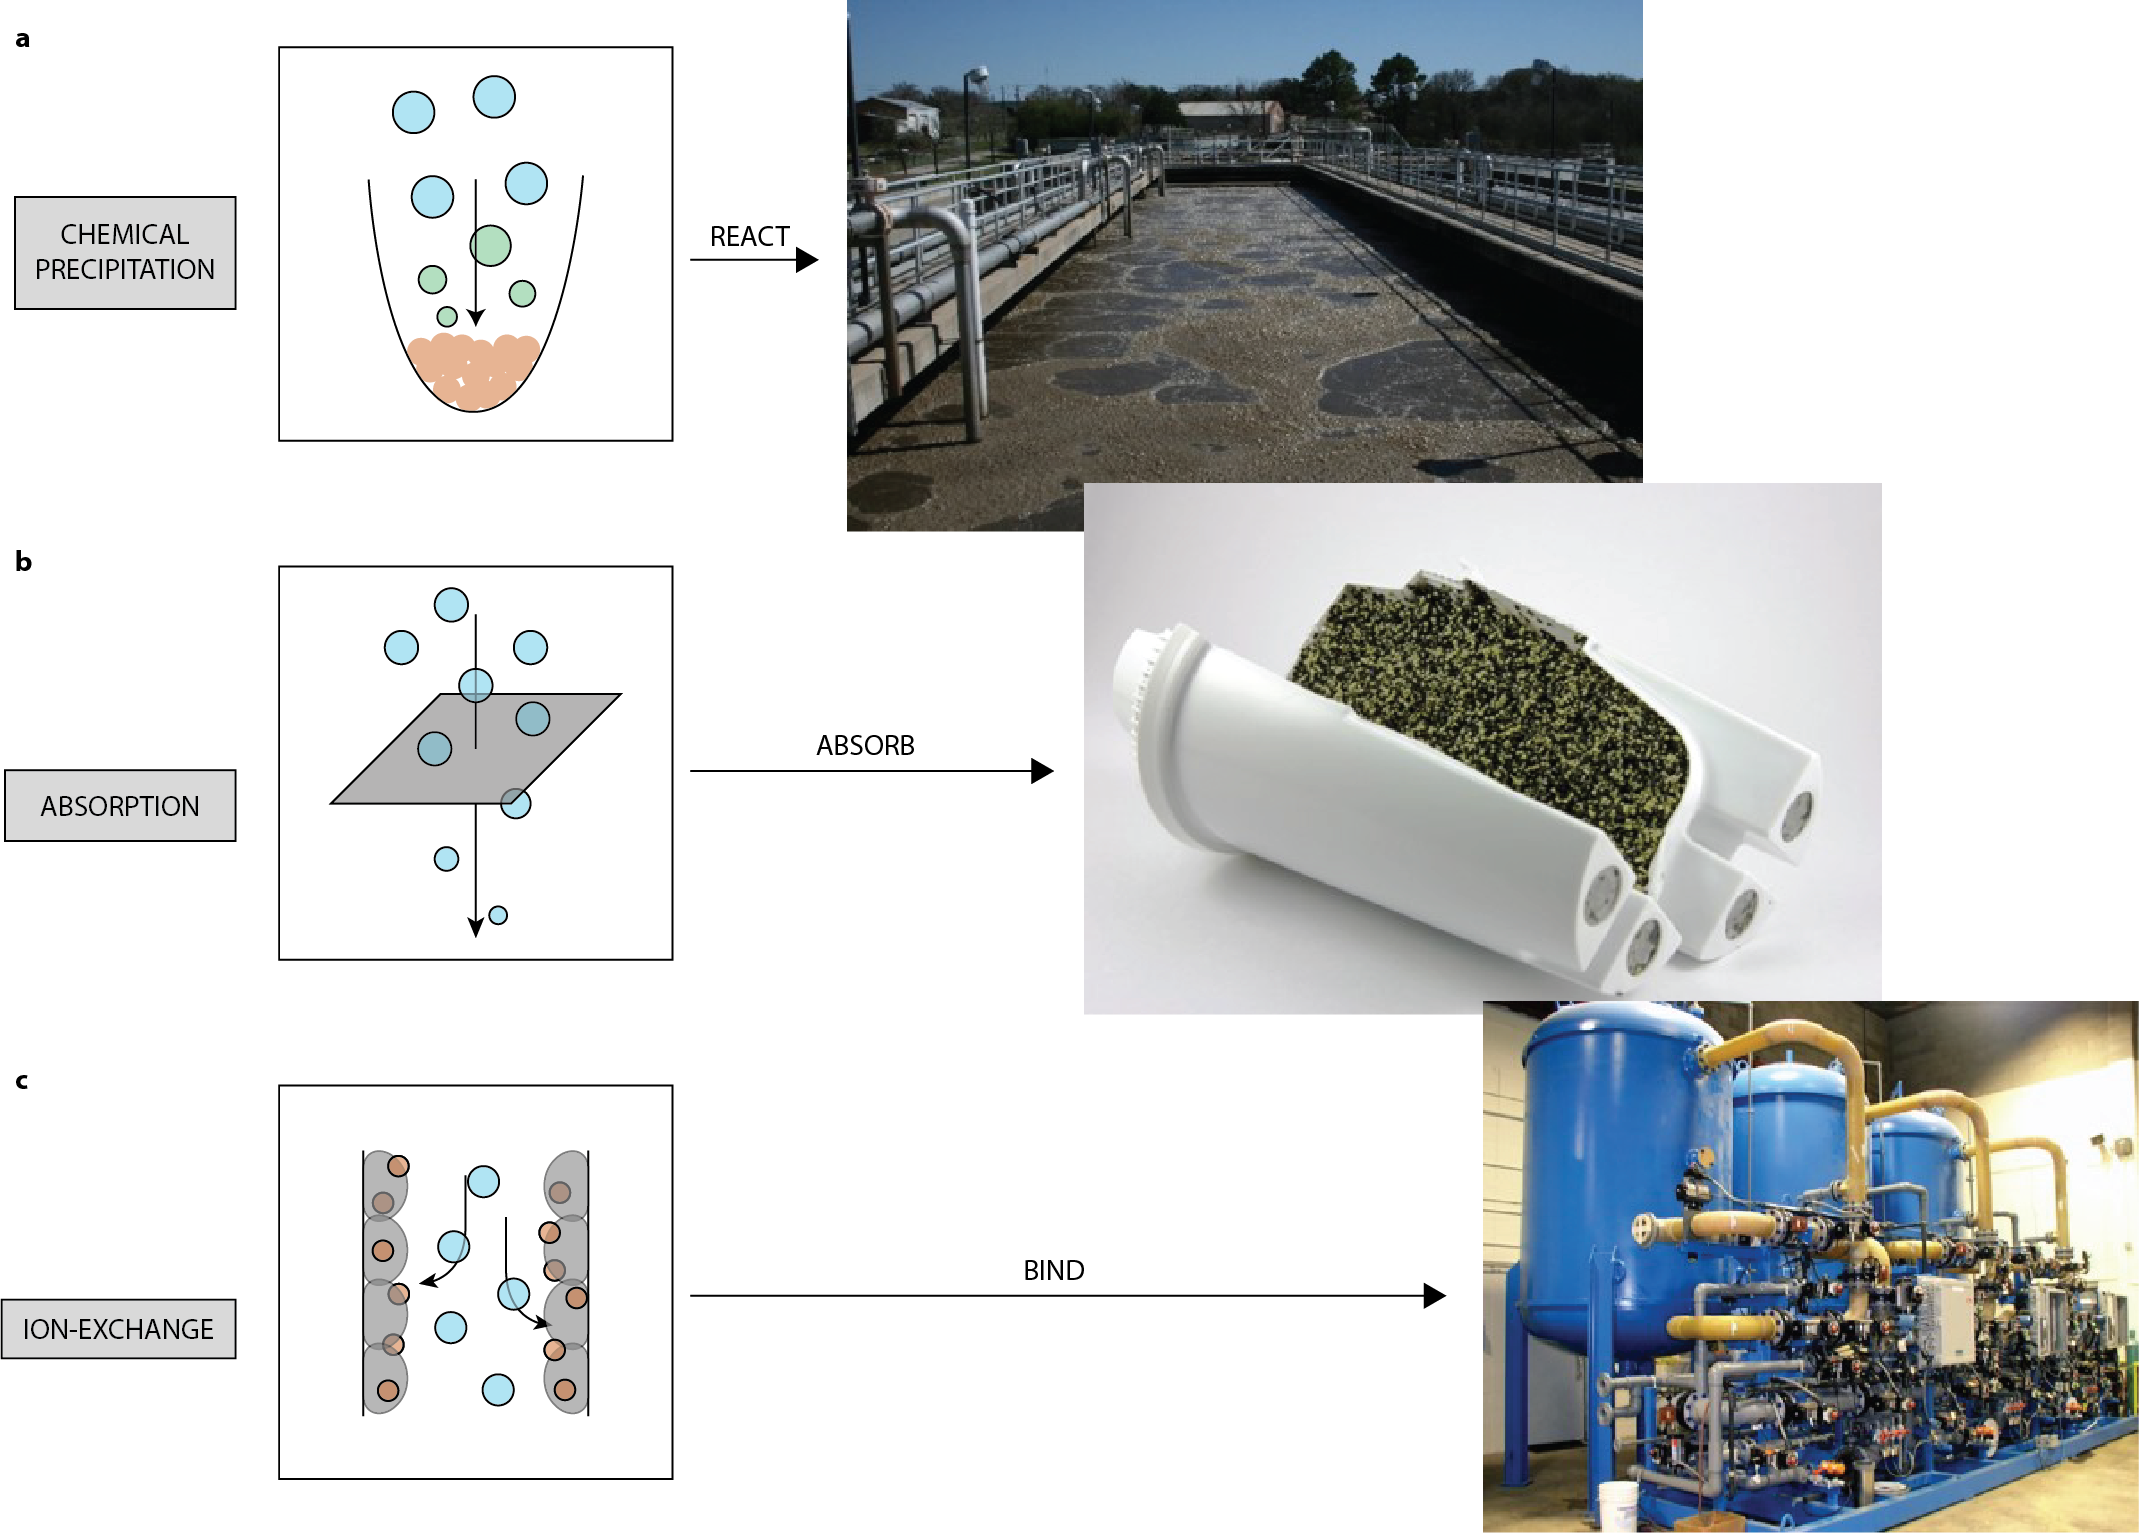
\includegraphics[width=\linewidth]{example-physicochemical.png}
	\caption[Overview of physicochemical processes used in industry]
	{
    \textbf{Overview of physicochemical processes used in industry}\protect\footnotemark.
    (\textbf{a}) Chemical precipitation relies on high pH and the addition of reactive species to precipitate metals from solutions. The benefit is the conversion of aqueous metals into solids which can be physically handled and removed.
    (\textbf{b}) Adsorption or absoprtion is the capture of metals onto or into a membrane or solid matrix, respectively. Well-known examples used in the market are activated carbon or synthesized semi-porous meshes.
    (\textbf{c}) Ion-exchange relies on the electrostatic interactions of metals and resins.  Resins are physically enclosed in columns or chambers in which waste water is poured into and eluted from. Metals captured can be later discharged from the resin and collected.
  }
	\label{figure:chapter1:example-physico}
\end{figure}
\footnotetext{
  Representative images of chemical precipitation, absorption, and ion-exchange come from online stock photos. All rights belong to their respective creators or owners.
}

%-----------------------------------------------------------------%
% SUBSECTION
%-----------------------------------------------------------------%
\subsection{Disadvantages and limitations}
Problems current physicochemical methods fail to address are cost, generation of secondary-waste, and technological accessibility. Almost all physicochemical processes require dedicated infrastructure to operate and manage. In addition, these processes require scientific skill and technical expertise to operate with regards to using reactors, synthesizing membranes or resins, or handling and storage of chemicals. Given these responsibilities it is extremely difficult for developing nations to adopt physicochemical technologies. Unfortunately, it is these same countries which have the most desperate need for economical and sustainable remediation technologies (\CHAPTER~\ref{ext-preface:rise-of-heavy-metal-waste}). Without a viable remediation technology, many countries are unable to manage their accumulation of waste. An investigation by the United Nations revealed that almost 80\% of global waste water is left untreated and allowed to flow back into drinking waters~\cite{unitednations2015,unu-inweh2017}. The problem is not the mechanism of action or removal efficiencies of current physicochemical technologies, but more so on the logistical and accessibility challenges that reduce the ease of adoption and use.

\subsubsection*{Chemical precipitation}
The precipitation of heavy metals is highly reactive and kinetically fast, allowing other particles to non-specifically aggregate within the precipitating mass~\cite{fu2011}. The result is the generation of amorphous sludge. Sludge is typically heterogenous and chemically ill-defined, inhibiting further processing or exctraction of individual elements. Therefore, typical disposal methods rely on dumping sludge into landfills or pyrolized~\cite{kurniawan2006,kumargupta2012}. Although chemical precipitation offers the convenience of extracting solid waste from the cleared liquid, the generation of sludge as a secondary-waste continues the cycle of ineffective waste treatment. Currently the handling and disposal of sludge is under investigation as an environmental and human health hazard~\cite{EPA_chemprecip_review}, as previously buried sludge is beginning to leach back into soil and public waters.

\subsubsection*{Absorption}
Heavy commercial use of current sorbent materials such as activated carbon have increased prices and significantly reduced availability. Research into new sorbents have been limited, as substituting materials such as carbon nanotubes and nanostructure materials are difficult to construct and are costly to synthesize~\cite{stafiej2007adsorption}. These barriers: cost, manufacturing difficulty, and material availability have limited widespread adoption of synthetic sorbent materials~\cite{fu2011}. Instead, there has been a push to discover natural sorbents such as rocks, minerals, and even composted biomass~\cite{razmovski2008biosorption}.

\subsubsection*{Ion-exchange}
Resin modifications are difficult to tailor per metal of interest, therefore monolithic chromatography columns are employed to indiscriminately capture free floating metal species. This method easily saturates resin beds with more abundant metals rather than metals that are rarer but acutely toxic (e.g. mercury versus sodium)~\cite{ustun2007regeneration}.
In addition, resin synthesis, column construction, and the need for dedicated fluid control infrastructure produces an added layer of logistical and technical difficulty for mainstream adoption. In addition, creating resins and modifying its metal-binding functional groups are difficult to engineer and can add cost to research and development~\cite{wachinski2016}. Often, the manufacture of resins produce secondary-waste in the form of chemical by-products during resin synthesis or regeneration of resins after use~\cite{amini2015}.

%===========================================================================%
% SECTION
%===========================================================================%
\section{New and developing tools in bioremediation}
Rather than focusing on man-made techniques for waste management, current research is moving towards cheaper and environmentally friendlier techniques which take advantage of natural waste processing strategies found in nature. Biologically-dervied or bio-inspired solutions are attractive methods because nature has already evolved numerous mechanisms for decomposing hazardous substances into less toxic or usable forms. The concept of waste management is universal in all biological systems, and these processes have been optimized in many organisms allowing them to survive in a variety of environments which are normally toxic to humans. The first example of utilizing biology for targeted remediation efforts was performed in the 1960s by George Robinson. Robinson demonstrated a bio-facilitated waste treatment reaction using bacteria to degrade petroleum and other polluting hydrocarbons~\cite{sonawdekar2012bioremediation}. Since then, the field has grown to include other natural and engineered organisms to react, absorb, and compartmentalize toxic metals. Until the 1990s, the methodology for designing bioremediation platforms was to engineer available microorganisms to enhance their tolerance and consumption of waste, specifically for oil and oil spills. However, as results did not improve during the years, from the 1990s onward scientists began to search for natural microorganisms that natively harbored desirable bioremediation characteristics~\cite{sonawdekar2012bioremediation,antizar-ladislao2010}. The discovery of new and exotic organisms became possible with the advent of new genetic and sequencing technologies.
Examples of adopted microorganisms are bacteria that live in highly corrosive volcanic vents to plants that thrive in polluted soils~\cite{bull2000search}.

%-----------------------------------------------------------------%
% SUBSECTION
%-----------------------------------------------------------------%
\subsection{Biological analogies to physicochemical processes}
\label{section:chapter1:biological-analogies}
Deconstructing the mechanisms behind physicochemical technologies, namely chemical preciptiation, absorption, and ion-exchange, reveal straightforward processes relying on fundamental scientific principles. Simply, these processes are to \textit{react}, \textit{absorb}, and \textit{bind} heavy metals away or out of contaminated waters. These mechanisms are not particularly unique to physicochemical processes. Biological systems routinely perform such functions to remove metals from their environments for survival purposes. In this work, several discoveries were made to find biological analogies to these physicochemical processes, and from there engineered for improved usability, scalability, cost effectiveness, and environmental sustainability~(\FIGURE~\ref{figure:chapter1:physico-versus-bio}).

%~~~~~~~~~~~~~~~~~~~~~~~~~~~~~~~~~%
% analogies of physico versus bio
%~~~~~~~~~~~~~~~~~~~~~~~~~~~~~~~~~%
\begin{table}[H]
\small
\centering
	\begin{tabular}{r c l}
	\toprule
	\makecell{Physicochemical process} & & Bioremediation equivalent \\
	\midrule
  chemical precipitation & $\rightarrow$ & biomediated mineralization \\
  adsorption & $\rightarrow$ & metal trafficking and cellular uptake \\
	ion-exchange & $\rightarrow$ & metal binders and cell surface display \\
	% electrochemical treatment & $\rightarrow$ & dissimilatory metal \& sulfur reduction\\
	\bottomrule
\end{tabular}

	\caption[Analogies between physicochemical and bioremediation strategies]
	{
		\textbf{Analogies between physicochemical and bioremediation strategies}
	}
	\label{table:chapter1:compare-physico-bio}
\end{table}

In a biological context, homeostatic balance of metal concentrations is essential---too much or too little will lead to cell death. Therefore, biology has evolved exquisite mechanisms to balance the flow of metals in to and out of a cell. Not surprisingly, the ability to react, absorb, and bind onto metals can be found in most biological systems (\TABLE~\ref{table:chapter1:compare-physico-bio}). These biological processes just come in another name; they are biomineralization, intracellular metal transport, and cell/protein mediated metal chelation.

%===========================%
% figure of physico vs bio
%===========================%
\begin{figure}[H]
	\centering
	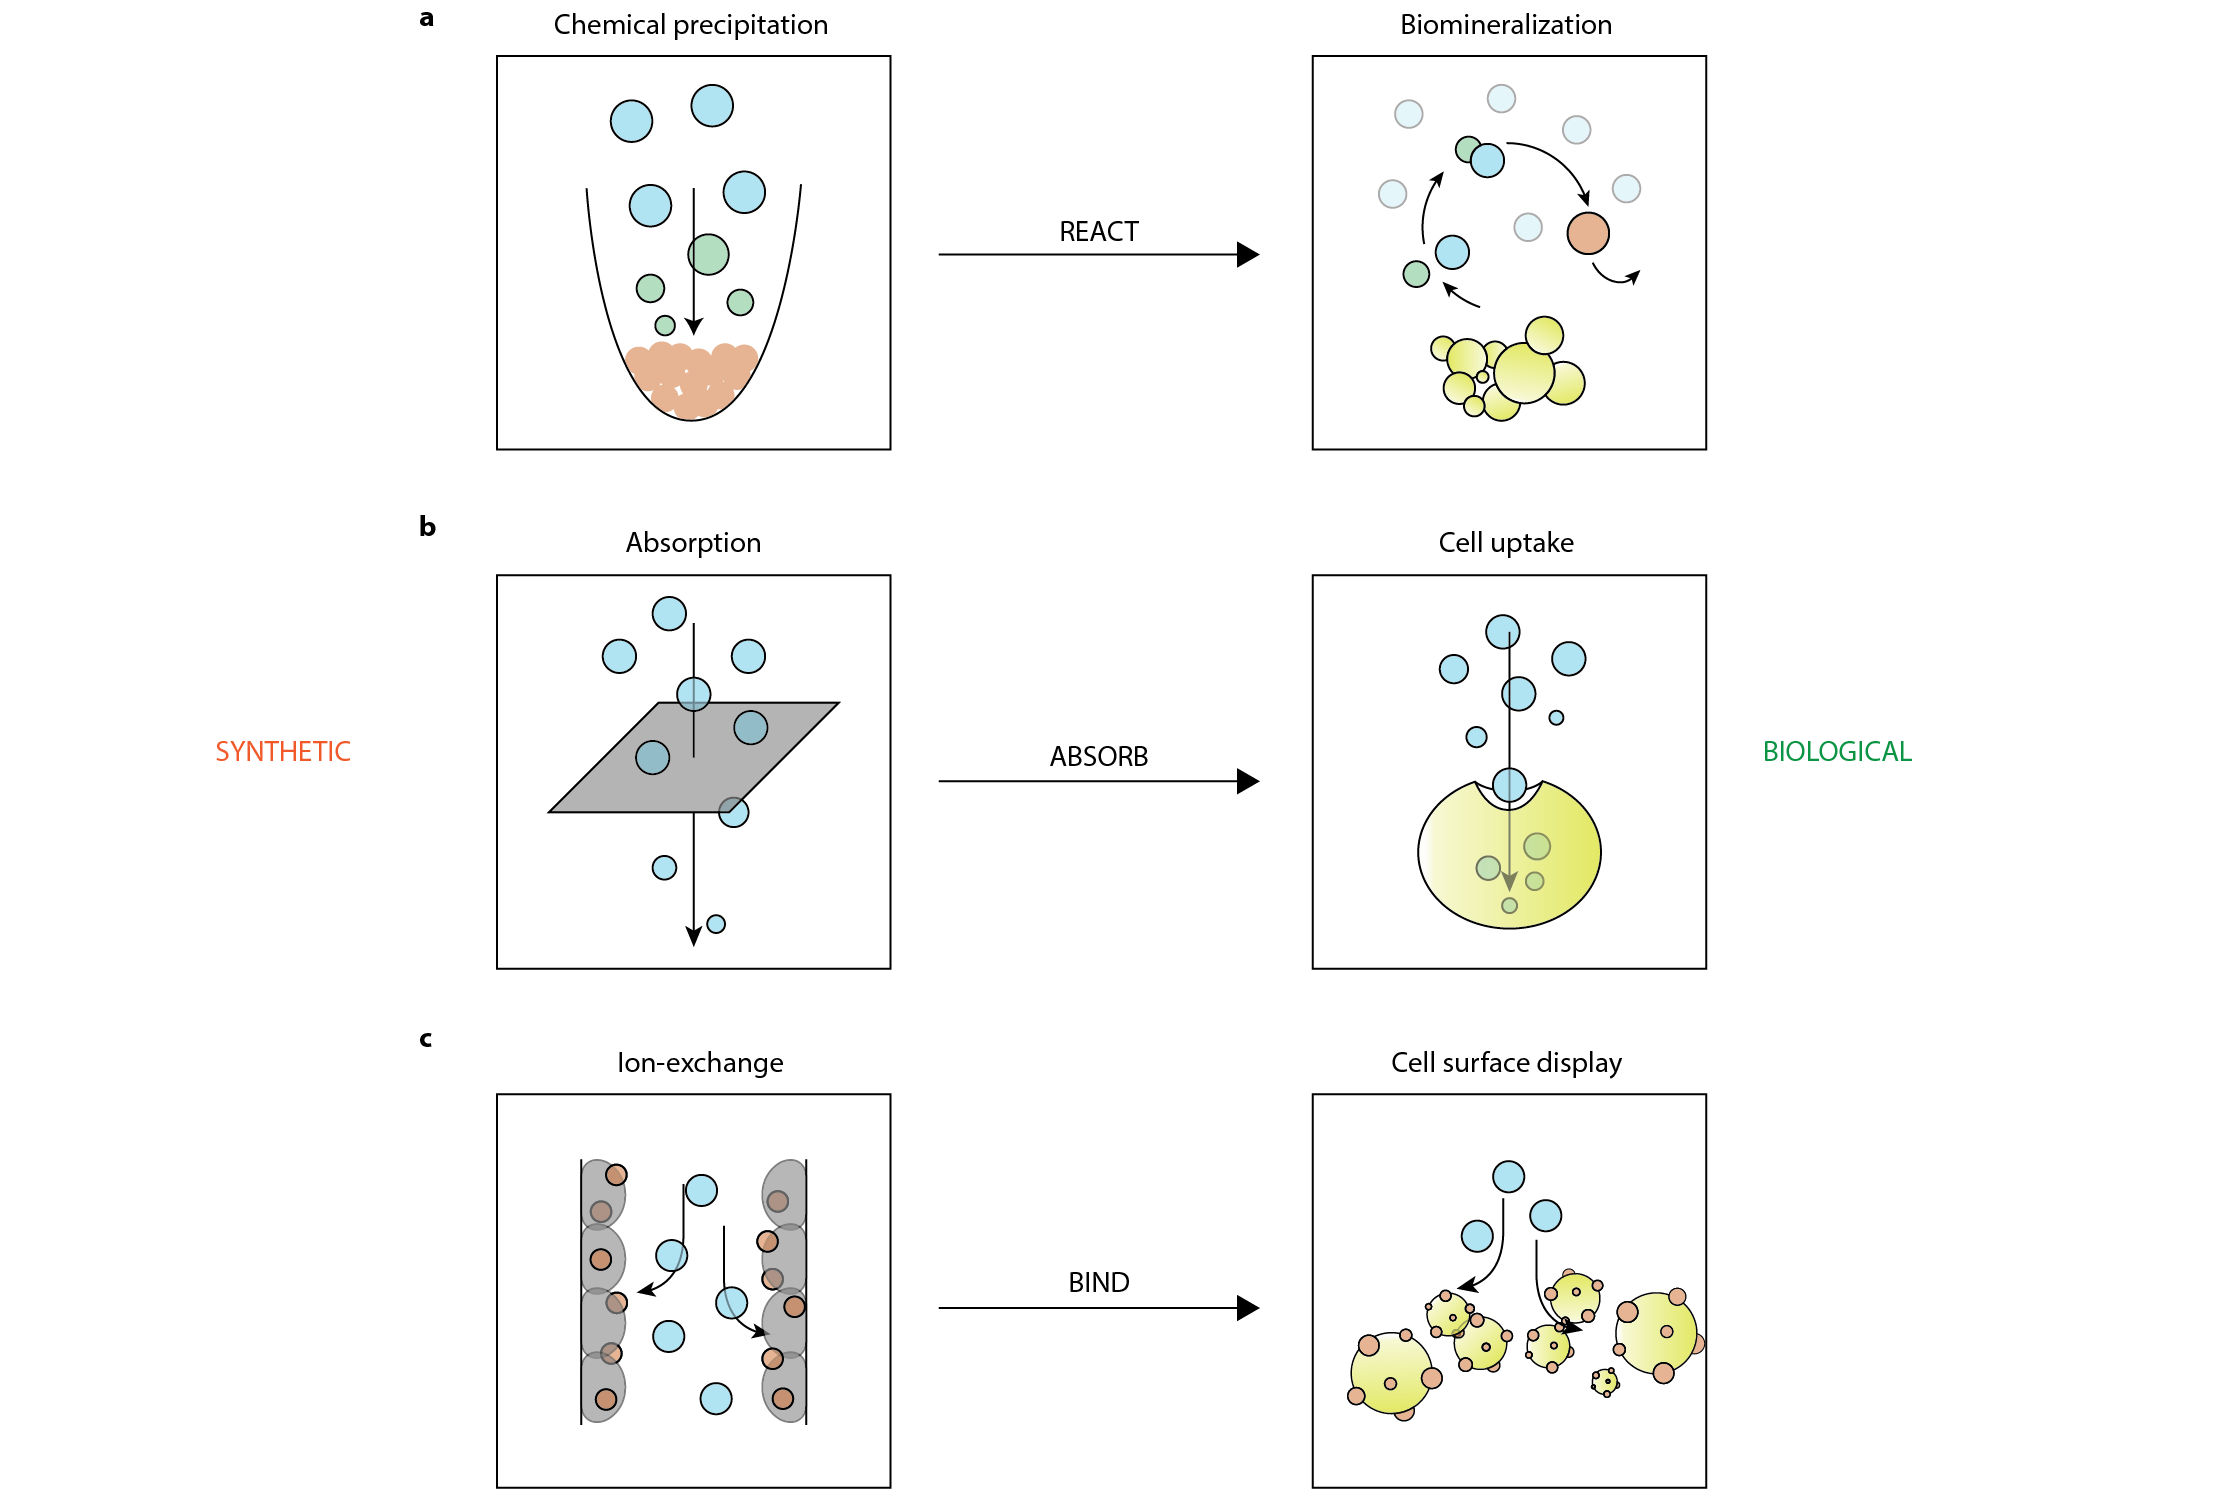
\includegraphics[width=\columnwidth]{physico-versus-bio.png}
	\caption[Analogies between physicochemical and biological processes for heavy metal removal]
	{
		\textbf{Analogies between physicochemical and biological processes for heavy metal removal}.
    (\textbf{a}) There are a variety of microorganisms that can produce their own chemicals for metal precipitation, a process commonly known as biomineralization. Examples are magnetosomes from magnetotactic bacteria, abalone shells, and diatom exoskeletons.
    (\textbf{b}) The intracellular volume of cells can be used as a compartment to absorb metals. Rather than manufacturing synthetic absorbing matrixes, biology can naturally grow their own.
    (\textbf{c}) The combination of cells and proteins can be used as a physical substrate to chelate and aggregate metals, much like in ion-exchange.
	}
	\label{figure:chapter1:physico-versus-bio}
\end{figure}
\clearpage % force a page break

%.......................................................%
% SUBSUBSECTION*
%.......................................................%
\subsubsection*{Biomineralization as an anology to chemical precipitation}
Biology has evolved unique strategies to coexist with inorganic materials, and in some instances, productively utilize these materials for biological purposes---bones, shells, exoskeletons, etc. The process to biologically synthesize and incorporate mineralized materials can be grouped into two modes, biologically induced mineralization (BIM), and biologically controlled mineralization (BCM)~\cite{frankel2003biologically}.

%==============================%
% Example - biomineralization
%==============================%
\begin{figure}[H]
	\centering
	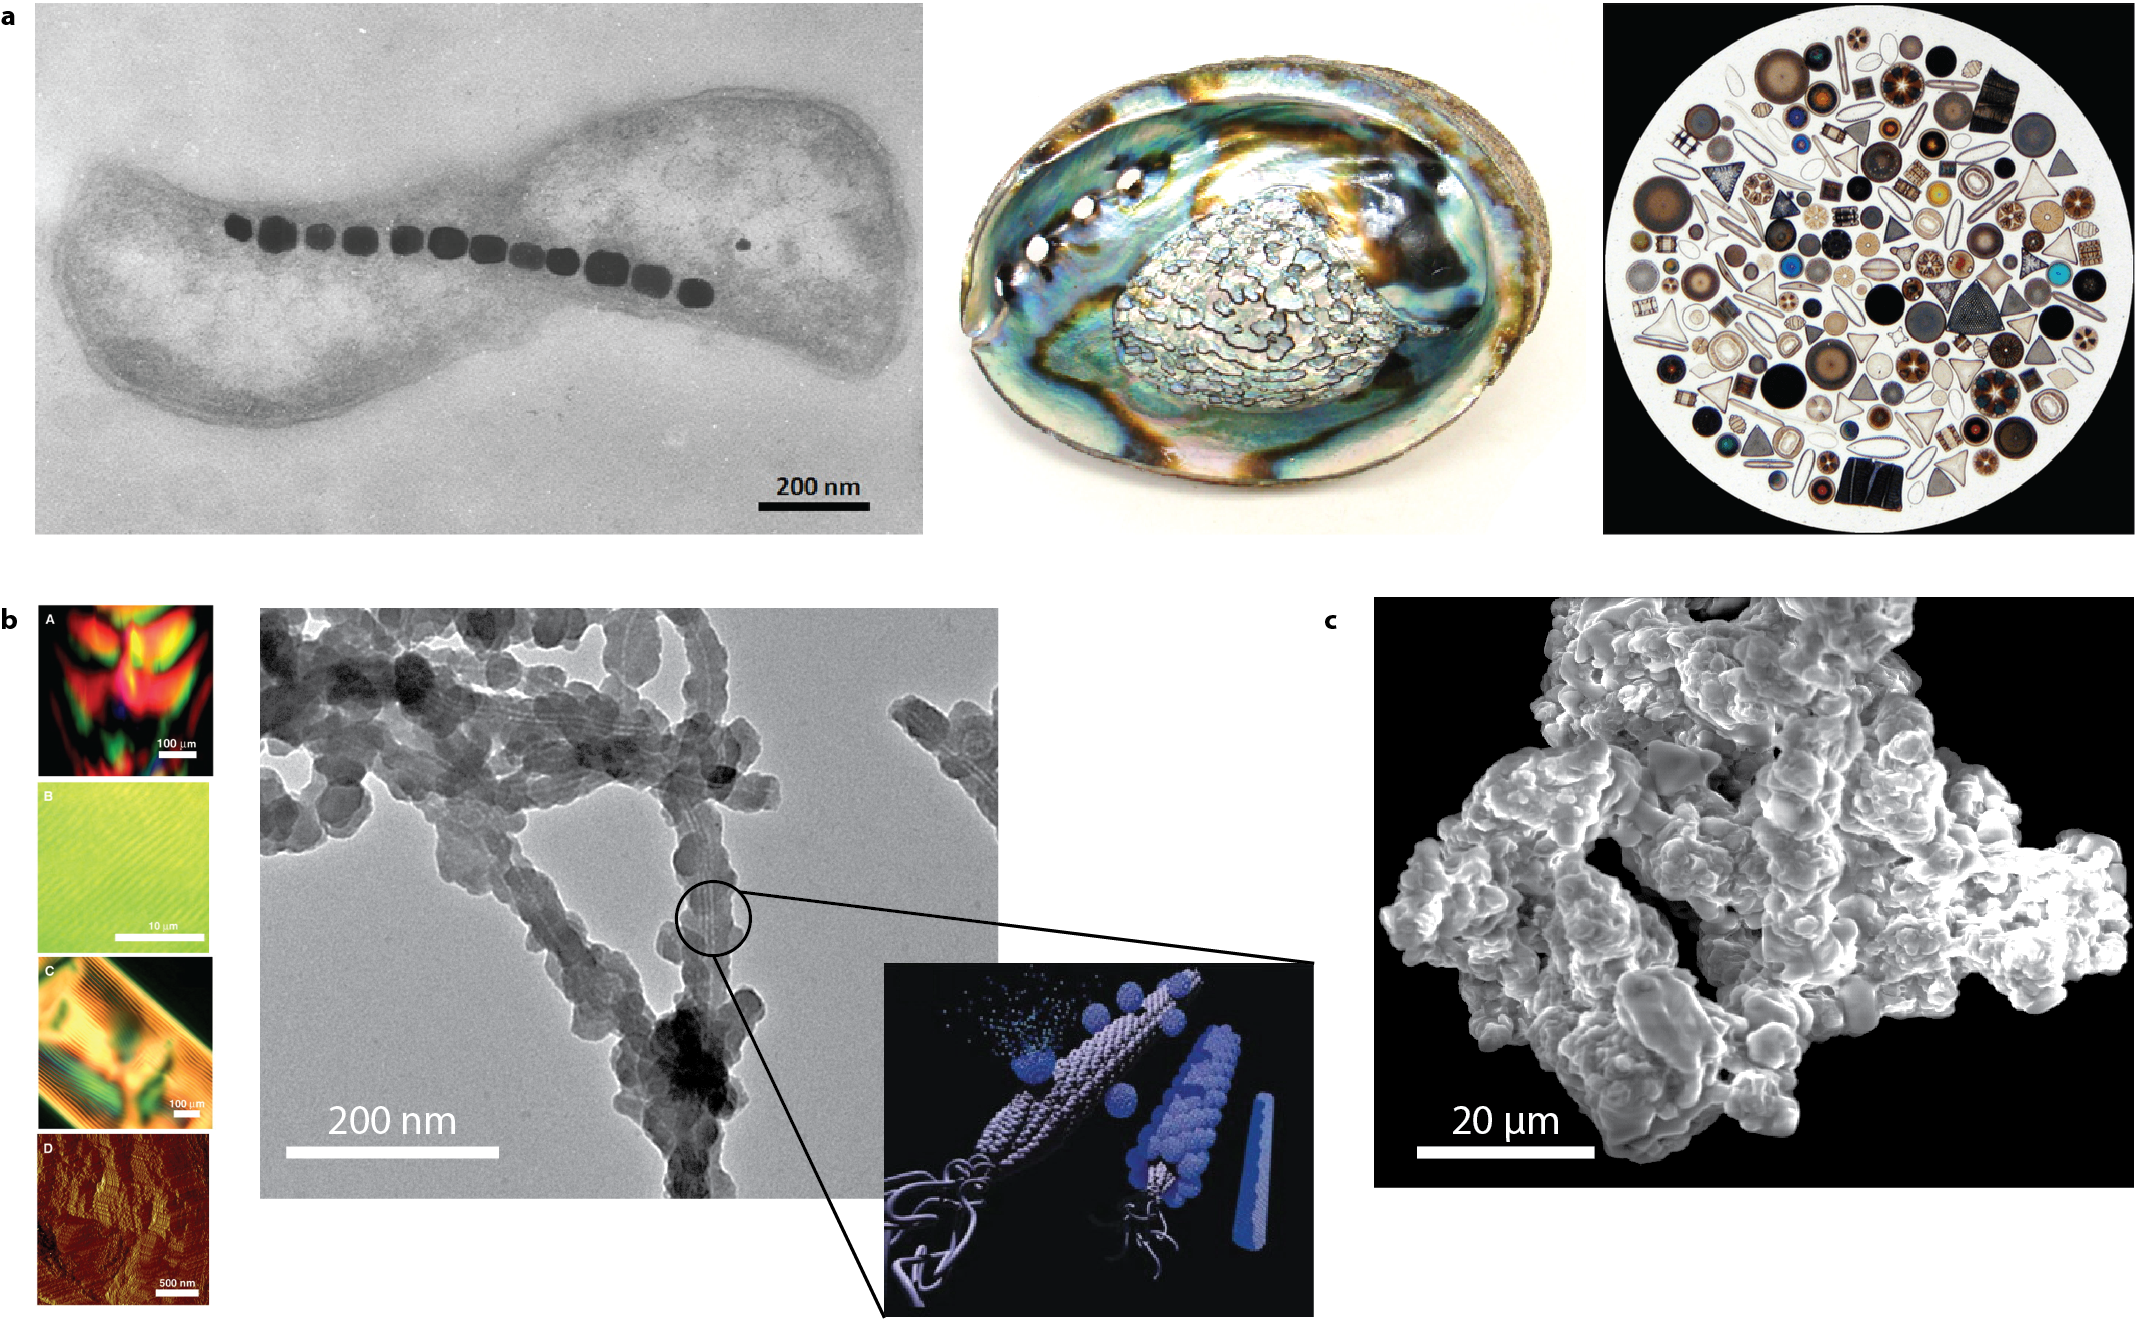
\includegraphics[width=\linewidth]{example-biomineralization.png}
	\caption[Natural and engineered biomineralization processes]
	{
		\textbf{Natural and engineered biomineralization processes}\protect\footnotemark.
    (\textbf{a}) (from left to right) Magnetotactic bacteria, abalone shells, and diatoms are examples of natural organisms that mineralize elements such as silicon, iron, and calcium to create biologically functional structures.
    (\textbf{b}) An example of phage used to template zinc sulfide nanocrystals to create quantum dot materials. (from left to right) Modifying the pVIII coating of the M13 bacteriphage allows controlled biominerlization alignment, as represented by the striations and color of the material. A TEM image of the underlying phage and coat material, with inset showing the process of templating phage with semi-conductor metals.
    (\textbf{c}) The same engineering approach to coat phage can be performed on other host organisms, such as yeast. SEM image shows yeast aggregated into a matrix of cells and \ce{CdS} nanoparticles.
	}
	\label{figure:chapter1:example-biomineralization-bio}
\end{figure}
\footnotetext{
  a) magnetotactic bacteria, abalone shell, and diatoms taken from Google images. All rights belong to their respective creators or owners.\\
  b) phage images taken from Lee, Seung-Wuk, et al. "Ordering of quantum dots using genetically engineered viruses." Science 296.5569 (2002): 892-895~\cite{lee2002ordering}.
}
\newpage % force a new page

BIM typically occurs for organisms that use metals as terminal electron acceptors which subsequently react and participate in mineral formation. BCM controls metal mineralization by facilitating growth in organic matrixes or vesicles within the cell (\FIGURE~\ref{figure:chapter1:example-biomineralization-bio}a). An organism discovered in the 1980s that has received incredible interest in the past decades is the magnetotactic bacteria~\cite{blakemore1982}. Magnetotactic bacteria are able to create magnetic particles in their bodies with extreme precision and control. Scientist are still uncovering the magnetosome formation mechanism, but research into this phenomenon shows that nature has found a way to naturally manufacture electromagnetic compounds with environmentally available minerals~\cite{uebe2016magnetosome}.

Using BIM and BCM, biological engineers have attempted to synthesize and create novel biologically derived materials for applications in semiconductor or biomaterial fabrication. A major breakthrough in bridging the gap betweeen organic and inorganic materials was performed by Lee et al. who demonstrated the BIM-like synthesis of \ce{ZnS} crystals on engineered M13 bacteriophage coat proteins (\FIGURE~\ref{figure:chapter1:example-biomineralization-bio}b)~\cite{lee2002ordering}. More so, other groups such as Tan et al. and Naik et al. have engineered small peptides to synthesize and control the formation of Au and Ag nanoparticles, respectively, in a BCM-like fahsion~\cite{tan2010uncovering,naik2002biomimetic}.

Alternatively, BIM and BCM-like processes can be exploited to precipitate and remove heavy metals from water. Through the use of phage and bacterial display, researchers have discovered peptides that nucleate minerals such as \ce{SiO2}, \ce{TiO2}, and \ce{Ca3(PO4)2}, and a comprehensive review by Chen et al. provides a table listing identified biomineralization peptides~\cite{naik2002silica,dickerson2008identification,gungormus2008regulation,chen2010peptide}.
Efforts to use biomineralization for the creation of novel materials can be equally applicable for metal precipitation and waste water remediation. These same peptides can be used to help mineralize and react metals from environmentally contaminated waters (\FIGURE~\ref{figure:chapter1:example-biomineralization-bio}c).

%.......................................................%
% SUBSUBSECTION*
%.......................................................%
\subsubsection*{Heavy metal transport as an analogy to adsorption}
Plants have evolved one of the more advanced mechanisms for heavy metal tolerance. As plants lack the ability to migrate away from toxic areas, they instead evolved robust defense mechanisms to absorb and sequester metals away from vulnerable tissues~\cite{hall2002cellular}. Plants that are able to preferentially absorb and accumulate metals are classified as hyperaccumulators. There are at least 400 species of identified hyperaccumulators. The defintion of hyperaccumulation being the accumulation of 100 mg/kg (0.01\% dry wt.) of cadmium or arsenic, 1000 mg/kg of (0.1\% dry wt.) of cobalt, copper, chromium, aluminum, nickel and lead, and 10,000 mg/kg (1\% dry wt.) of manganese, iron, and zinc~\cite{rascio2011heavy,vara2003metal,branquinho2007revisiting,kramer2010metal}.

A review by Clemens et al. highlights the significance of metal transporters and chelating agents in contributing to plant's hyperaccumulating capabilities~\cite{clemens2002long}. Hypothesized transporters implicated in hyperaccumulation are
CDFs (\underline{c}ation \underline{d}iffusion \underline{f}acilitators), special classes of passive transporters such as
ZIPs (\underline{Z}RT and \underline{I}RT-like \underline{p}roteins),
Nramps (\underline{n}atural \underline{r}esistance \underline{a}ssociated \underline{m}acrophage \underline{p}roteins),
heavy metal ATPases, and
ABCs (\underline{A}TP \underline{b}inding \underline{c}asettes)
(\FIGURE~\ref{figure:chapter1:example-transporter})~\cite{clemens2002long,kramer2010metal}.

%===========================%
% figure of transporters
%===========================%
\begin{figure}[H]
	\centering
	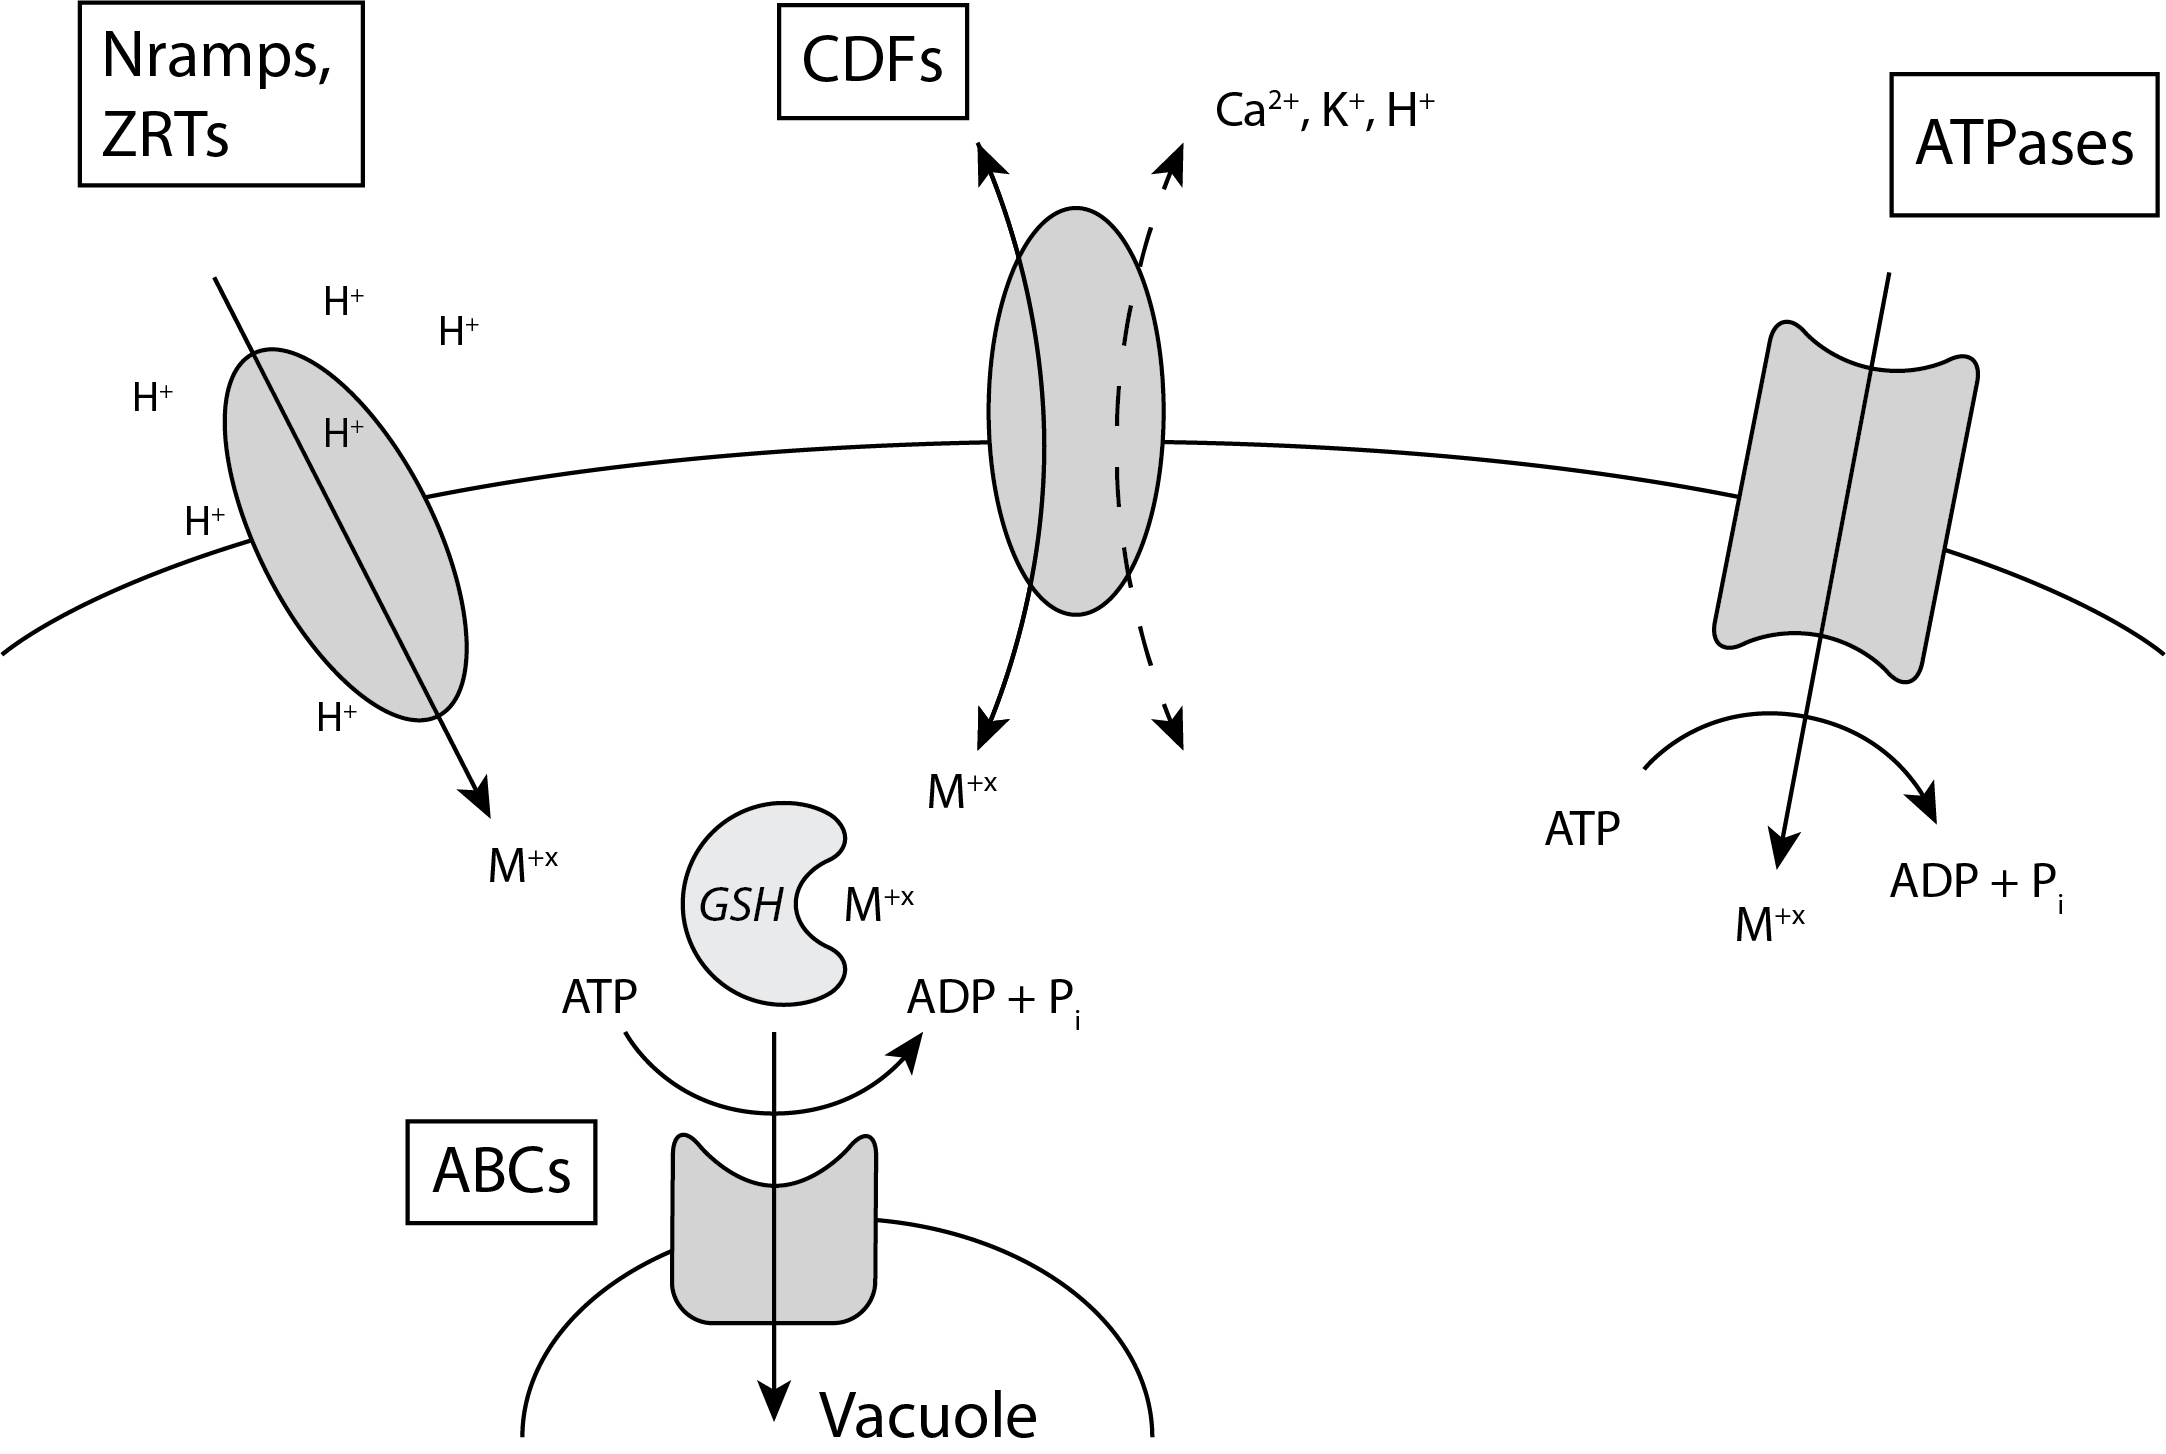
\includegraphics[width=0.66\columnwidth]{example-transporters.png}
	\caption[Overview of metal trafficking and sequestration mechanisms in plant cells]
	{
		\textbf{Overview of metal trafficking and sequestration mechanisms in plant cells}
	}
	\label{figure:chapter1:example-transporter}
\end{figure}

Further work by Clemens et al. demonstrated that the ZIP family contributes to \ce{Fe^{2+}} and \ce{Zn^{2+}} hyperaccumulation, whereas the Nramp families have a broad spectrum of metal uptake capabilities~\cite{clemens2001molecular}. On the other hand, Pittman et al. showed that knockouts of antiporters, namely members of the CDF family led to hypersensitivity and hyperaccumulation of \ce{Zn^{2+}}, \ce{Co^{2+}}, and other trace metals~\cite{clemens2002transporter,pittman2005managing}.
ABC transporters have recently been shown to transport metals into vacuoles after intracellular uptake, and it is hypothesized that ABC transporters recognize metal-phytochelatin complexes (e.g. glutathione or trypanothione) which they then carry into vacuoles as phytochelatin-mediated conjugates~\cite{hall2003transition,legare2001leishmania}.

%~~~~~~~~~~~~~~~~~~~~~~%
% list of transporters
%~~~~~~~~~~~~~~~~~~~~~%
\begin{table}[H]
\small
\centering
	\begin{tabular}{l l l p{4cm}}
	\toprule
	Transporter & \makecell{{\centering}Metal} & Where & \makecell{Requires} \\
	\midrule
	CDF & Mn/Fe/Zn/Co/Cd & varies & antiports counter ions\\
	ZIP & Fe/Zn & membrane & proton gradient \\
	Nramp & Fe/Zn/Mn/Co/Ca/Cu/Ni/Pb & membrane & antiports \ce{H^+}\\
	ATPases & Cu/Ag/Zn/Cd/Pb/Co/Ca/Mg & membrane & ATP \\
	ABCs & phytochelatin + metal complex & vacuole & ATP \\
	\bottomrule
\end{tabular}

	\caption[Transporter types listed by preferred metal, localization, and mechanism of action]
	{
		\textbf{Transporter types listed by preferred metal, localization, and mechanism of action}
	}
	\label{table:chapter1:transporters}
\end{table}

The ability to uptake and compartmentalize metals also enables elevated tolerance to toxic levels of environmental metal concentrations. Tolerance is primarily due to compartmentalization inside vacuoles~\cite{song2010arsenic} or binding from sequestration agents such as phytochelatins or metallothioneins~\cite{cobbett2002phytochelatins}. Phytochelatins are oligmers of glutathione (GSH; $\gamma$Glu-Cys-Gly), and metallothioneins (MTs) are a family of cysteine-rich low molecular weight proteins. Both species utilize cysteine's thiol group to sequester heavy metals, and both have promiscuous binding affinities for mono- and divalent metals such as Zn, Hg, Cu, As, and Ag~\cite{cobbett2002phytochelatins}. Overall, metal accumulation in plants is possible due to a combination of hyperactive transporters and a defense network of metal chelating molecules.
\clearpage % force page break

%.......................................................%
% SUBSUBSECTION*
%.......................................................%
\subsubsection*{Protein-metal chelation as an anology to ion-exchange}
Ion-exchange modifies the surface chemistry of resins to electrostatically bind onto metals. The same technique can be done for cell surfaces, in which the exterior cell wall or membrane can be biochemically modified to display chelating moieties for metal capture. This technology called cell surface display has been engineered in several hosts such as bacteria and yeast in which an extracellular anchor (in bacteria LamB/OmcAl; yeast AGA1/2) is fused to a protein of interest (POI) (\FIGURE~\ref{figure:chapter1:example-biomineralization-bio}a)~\cite{freudl1986cell,boder1997yeast}. The POI is then tethered to the cell wall or membrane thereby decorating the surface for extracellular binding.
From this point of view, a cell is no different than a resin bead; sizes are approximately 1--10 $\mu$m in diameter, and both surfaces can be functionalized with various metal binders (\FIGURE~\ref{figure:chapter1:example-biomineralization-bio}b).

The advantage of using cell surface display rather than ion-exchange is that displayed proteins can be easily engineered and modified. Additionally, cell production is autonomous, easily stored and handled, and the resources needed to maintain large quantities of cells may be more cost-effective than handling synthetic compounds. In addition, surface binding proteins can be engineered to become highly sensitive and selective for a specific metal through high-throughput screens and/or directed evolution~\cite{peelle2005}. A common challenge for ion-exchange is the saturation of resin beds with more abundant metals, such as sodium, over highly toxic yet less abundant heavy metals such as mercury. In a biologically-derived system it is possible to engineer protein-metal interactions to be highly selective, thereby reducing interference of background metals during the remediation process.

Recently, work performed by Ruta et al. functionalized the yeast surface with hexapeptides to capture a range of common divalent metals such as Ni, Cu, Fe, etc~\cite{ruta2017}. In addition, cells with displaying metal binding proteins tend to be more metal tolerant, as metal captured extracellularly are prevented from entering the cell body~\cite{ruta2017,kuroda2001cell}. However, current literature data show low binding capacities in the $\mu$M range and poor capture to cell weight ratio compared to ion-exchange resins. Binding capacities on a per weight scale for ion-exchange is 3--6 orders of magnitude greater than using bacteria or yeast display technologies~\cite{barakat2011new,stathi2010heavy}. Therefore the number of binding sites per cell is the greatest limiting factor in removing an impactful amount of metals per volume, and so far display technologies for waste removal has not been able to overcome this limitation.

%=========================%
% Example - yeast display
%=========================%
\begin{figure}[H]
	\centering
	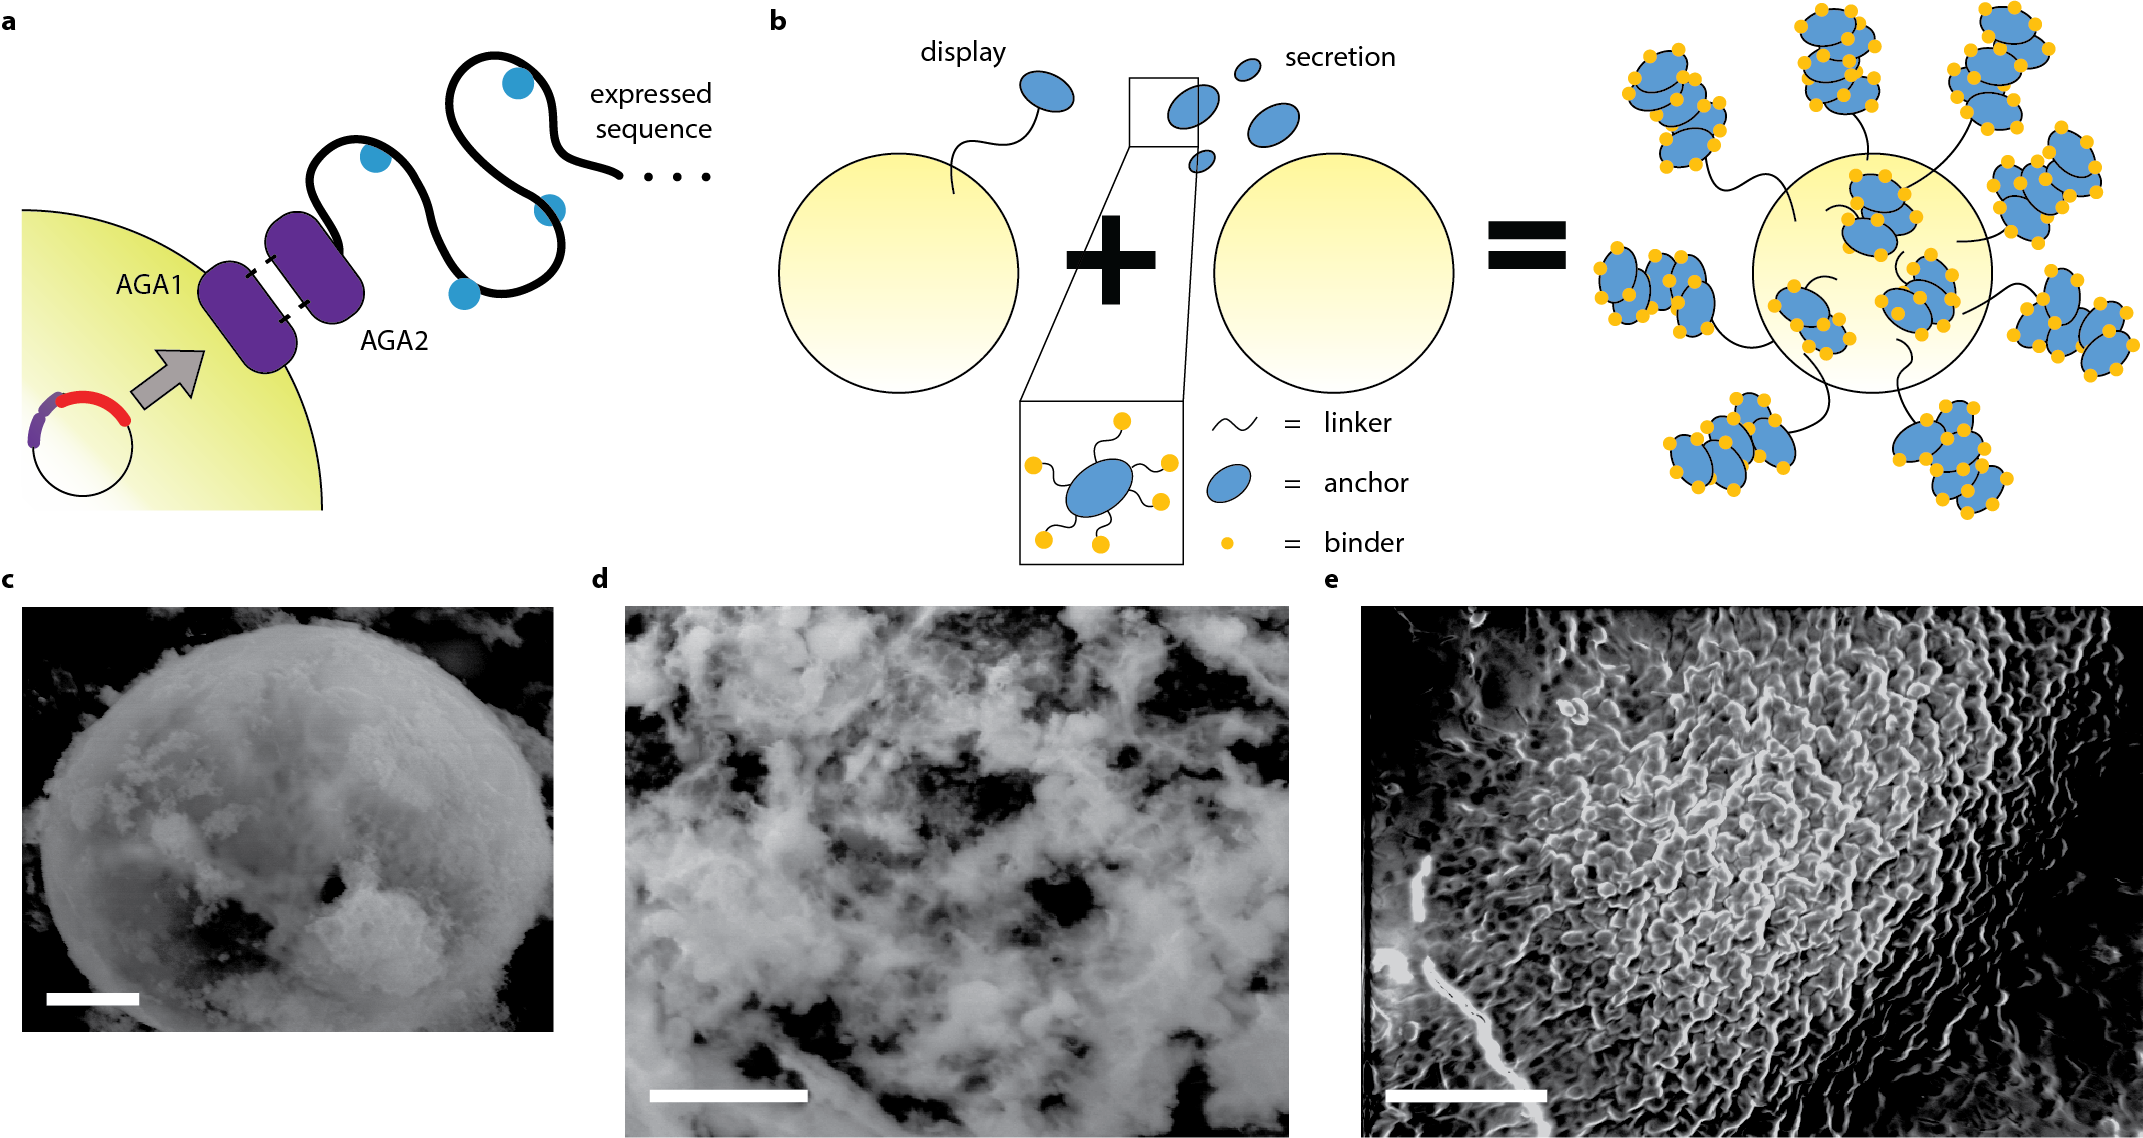
\includegraphics[width=\linewidth]{example-display.png}
	\caption[Using cell display and protein-metal binding technologies to remove metals]
	{
		\textbf{Using cell display and protein-metal binding technologies to remove metals}.
    	(\textbf{a}) Example schematic of yeast display using the AGA1/2 system for display of metal binding peptides. Purple ovals represent the AGA1/2 anchoring domains, and blue spheres represent areas of metal binding.
    	(\textbf{b}) To improve metal binding capacities, a system with yeast could both (or simultaneously) secrete and display aggregating proteins (blue) fused with metal binding moieties (orange) to effectively increase the surface number of metal binding domains. Rather than with traditional display technology of a single peptide/protein molecule per display, this system allows for multiple displayed domains to be anchored onto the cell surface.
    	(\textbf{c}) Example of yeast display bound to precipitated copper metal. Scale bar represents 1 $\mu$m.
			(\textbf{d}) Example of yeast display with aggregating proteins to create a yeast-protein matrix for metal binding. Scale bar represents 10 $\mu$m.
			(\textbf{e}) A hybrid approach in which yeast that display and secrete aggregating proteins are embedded in a bacterial biofilm for metal capture\protect\footnotemark. Nodules represent cluster of yeast colonies. Scale bar represents 50 $\mu$m.
	}
	\label{figure:chapter1:example-biomineralization-bio}
\end{figure}
\footnotetext{
	sample preparation and image taken with Zijay Tang from the Tim Lu Lab, MIT.
}

%-----------------------------------------------------------------%
% SUBSECTION
%-----------------------------------------------------------------%
\subsection{A reason for biology, and the focus on yeast}
Biology has provided a gambit of organisms and biological pathways to handle and utilize metal compounds in the environment. However, there is no one microorganism that can provide all of the functionality described above (\SECTION~\ref{section:chapter1:biological-analogies}). Therefore a candidate microorganism needs to be selected for further engineering.

However, rather than taking a bottom-up approach in which requirements and design criterias are first drafted and tested per microorganism of interest, this study focuses on a top-down approach in which high level specifications such as cost, scalability, and engineerability are first considered to then narrow in on a candidate microorganism.

%=========================%
% Venn diagram - yeast
%=========================%
\begin{figure}[H]
	\centering
	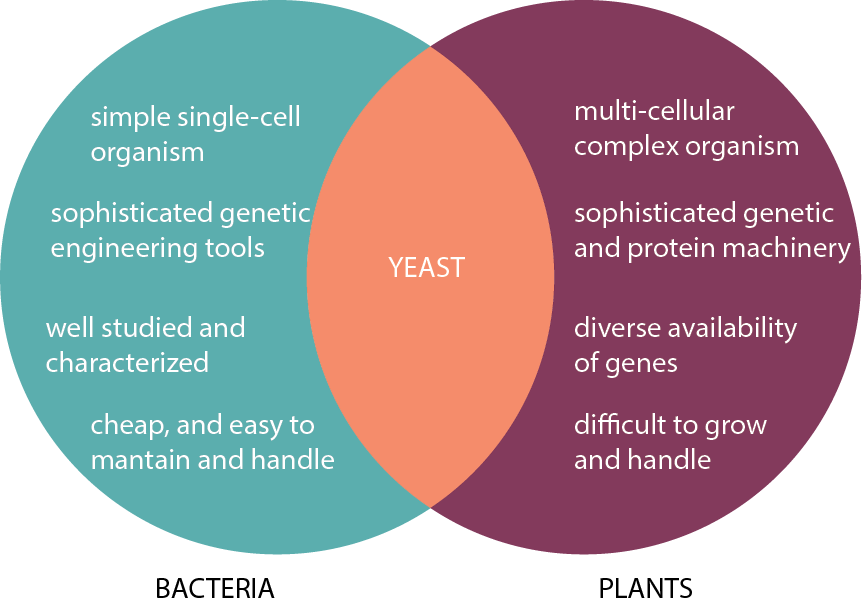
\includegraphics[width=0.5\linewidth]{venn-diagram-compare-organism.png}
	\caption[Advantages and disadvantages of using bacteria, yeast, or plants as a model organism for waste remediation research]
	{
		\textbf{Advantages and disadvantages of using bacteria, yeast, or plants as a model organism for waste remediation research}.

	}
	\label{figure:chapter1:venn-diagram}
\end{figure}

So far the high-level organismal categories routinely used in biological studies are bacteria, yeast, and plants. Bacteria, specifically \textit{Escherichia coli} have been the model organism for biological studies given their ease to grow, well understood cellular mechanisms, and sophisticated genetic and protein engineering technologies that were built on centuries of research. However, bacterial systems may be too simple of a starting point to build a complete remediation strategy. The advent of synthetic biology is bringing in a new wave of hybrid bacterial systems to counter this notion, but many of the technologies in genetic circuits and directed evolution are still maturing~\cite{blount2012construction}. Plants on the other hand, namely the model organism \textit{Arabidopsis thaliana}, have already proven themselves to be useful players for waste water remediation~\cite{rascio2011heavy}. Yet unlike bacteria, plants are difficult to grow and maintain given their diverse growing conditions. Especially, plant genetic and protein engineering technologies have yet to reach the maturity of bacterial based systems primarily because of the complexity of plant cellular biology.

Given the almost two opposite ends of bacteria and plant biology, what is almost a goldilocks compromise between the two model organisms \textit{Saccharomyces cerevisiae}---the common baker's yeast (\FIGURE~\ref{figure:chapter1:venn-diagram}). It can be argued that yeast were the first microorganism to be deliberately used by man, specifically for food and beer~\cite{greig2009,spencer1997}. Like bacteria, yeast have a mature biotechnology platform in which strains are routinely engineered, and not just for research purposes, but also for the consumer and pharmaceutical applications~\cite{nielsen2013,chae2001}. But unlike bacteria, yeast are eukaryotic organisms that contain sophisticated metabolic machinery and have a variety of protein homologues that are shared between both bacteria and plants.
More so, the past centuries of yeast-based research has unveiled almost an enclcyopedia knowledge of yeast genomic, proteomic, and metabolic profiles~\cite{guthrie2002guide}. Such a spectrum of information is still unavailable for plants, as plants are much more diverse with more complex biology. Therefore yeast seems to be the best compromise between the two platforms.

Aside from the technology, yeast also come with logistical advantages. Yeast have been used for almost 5000 years~\cite{greig2009}, and now it has become a common house-hold item that touches all areas of the globe integrating into many national, ethnic, and cultural backgrounds. Yeast-based consumer goods are routinely FDA approved~\cite{nutrition2018,usda2014}, and the global scaling and reduced cost of yeast has been pioneered by the food and beer industries.

Herein, this work shows that yeast can be a robust and tunable platform for next generation bioremediation technologies. Not only that, the technologies derived in this study are meant to translate into the yeast consumer market, where the same technologies used to make bread and beer can be leveraged to clean today's rise in waste waters.

%===============================BIBLIOGRAPHY================================%
\printbibliography[title=References]

\end{document}
